
\documentclass{book}
\usepackage{a4,makeidx,fancyheadings}
\usepackage{graphicx}
\usepackage[francais]{babel}
\usepackage[utf8]{inputenc}
\usepackage{fancyvrb}
\usepackage{makeidx}
\usepackage{tabularx}
\usepackage{eurosym}
\usepackage{color}
\usepackage{url}
\usepackage{pdfpages}
\usepackage{geometry}
\geometry{ 
      hmargin=3cm,
      vmargin=3cm
}

\makeindex
	
\begin{document}
\newcommand{\motcle}[1]{\index{#1}\emph{#1}}
\newcommand{\instrcle}[1]{\index{\texttt{#1}}\texttt{#1}}

\thispagestyle{empty}
%-------- fancy headings setting -----------
\rhead[]{}
%\footrulewidth 0.1pt
\rfoot[]{\small\sc S. Genaud}
\pagestyle{fancy}
%------------------------- Page de Garde -------------------
\setlength{\parindent}{0mm}
\setlength{\parskip}{0mm}
\vspace*{\stretch{1}}
\rule{\linewidth}{1mm}
\begin{center}
\Large{Audit du Système d'Information}\\[5mm]
\Large{de l'Ecole de Management de Strasbourg}\\[5mm]
\large{Stéphane Genaud}
\rule{\linewidth}{1mm}
\vspace*{\stretch{2}}
\end{center}
\begin{center}
juin \oldstylenums{2011} \\
\textrm{
$Revision$\\
$Id$\\
$Date$\\
}
\end{center}
%------------------------------------------------------------

\tableofcontents
\newpage

 
 

\chapter{Services Audités}
 

\section{Responsable Informatique}

\paragraph{Christos Karakostas} (Responsable)


\section{Recherche}
\paragraph{Karine Bouvier (KB), Maxime Merli (MM), Thierry Nobre (TN)}

\subsection{Processus fonctionnels}

Le besoin quasi-exclusif est le recensement des publications des chercheurs.
Cette information sert à deux types processus:
\begin{itemize}
\item[$\bullet$] RC-1) L'évaluation de la production scientifique individuelle ou 
collective (AERES, accrédiations, classements, etc).
\item[$\bullet$] RC-2) La communication sur les centres d'intérêts et compétences 
vers l'extérieur (sites web, faculty book, etc).
\end{itemize}

\bigskip
L'information doit être structurée de façon à répondre aux exigences des 
différentes instances d'évaluations (AERES, organismes d'accréditation).
Cette structuration des informations bibliographique est classique et des
formats existent depuis longtemps (par exemple bibtex). Une spécificité
à prendre en compte est les classements des revues établi annuellement par 
l'AERES.

D'autres processus peuvent être identifiés, comme par exemple l'organisation
d'une conférence, où la collecte d'information concernant le devenir des
doctorants. Cependant, l'essentiel de ces actions sont ponctuelles et ne 
nécessitent pas un support récurrent du système d'information. La seule 
activité récurrente annexe identifiée est la consultation de l'état des 
finances. Dans ce cas, l'interface web avec SIFAC ainsi que les contacts 
nécessaires avec le gestionnaire des comptes apparaissent satisfaisants.



\subsection{Existant}

L'existant est essentiellement constitué de:
\begin{itemize}
\item la base de données recherche (MS Access), propre à l'EM,
\item l'application, partie de l'intranet, qui gère cette base : saisie, 
modification, consultation de la base.
\end{itemize}
Un premier projet a été mené en 2010 pour constuire cette base de données des
publications des enseignants-chercheurs de l'EM Strasbourg. Il a été demandé à 
CK de développer une fonctionnalité de l'intranet pour cela. L'interface de 
saisie développée n'étant pas assez contrainte, ce premier projet n'a pas 
permis de collecter des données d'une qualité suffisante pour être exploitables
pour produire les statistiques requises (e.g noms de revues orthographiées 
différement). Sur la base de ce constat, l'outil de collecte a été amélioré en 
2011. Du point de vue des responsables du projet (MM, KB, TN) l'outil donne 
satisfaction en ce qui concerne la qualité des données. Des fonctionnalités 
supplémentaires sont envisagées de manière non urgente (fichier PDF téléchargeable 
de la publication, remontée automatique du papier sur des archives ouvertes comme SSRN%
\footnote{\url{ http://www.ssrn.com/}}).
La façon dont les informations sont présentées sur les pages web personnelles
des enseignants-chercheurs%
\footnote{\url{http://www.em-strasbourg.eu/enseignants/em-strasbourg-enseignants}}
est également jugé satisfaisant.


\subsection{Analyse}

Il ressort de la discussion que les principaux problèmes auxquels ont eu à 
faire MM et KB pour la mise en place du projet sont:
\begin{itemize}
\item un problème d'interlocuteur : ils n'ont pas trouvé de personne référente 
capable de les orienter sur les ressources internes ou externes, capables de fournir 
la prestation dont ils avaient besoin.
\item un problème de conduite de projet : une fois la ressource chargée de la 
réalisation identifiée (CK), leur demande n'a pas fait l'objet d'une conduite
de projet. La planification était hasardeuse, le cahier des charges et
les validations peu formalisées.
\end{itemize}

\paragraph{Qualité des applications}
Il est à noter que l'interface construite ne permet pas de faire d'import (bibtex, 
endnotes,~...). 

\paragraph{Bilan qualité des données}
~\\


	\begin{tabular}{|l|l|l|l|l|l|l|}
	\hline
	efficacité	& efficience &	confidentialité	& intégrité & disponibilité & conformité & fiabilité \\
	\hline
	
	\hline
	\end{tabular}
	


%--------------- Relations Entreprises -----------------------------------

\section{Relations Entreprises et EM Strasbourg Partenaires}

\paragraph{Marie-Hélène Brémont (MHB), Hélène Heintz (HH), Francis Schillio (FS)}
~\\

\textit{Le service Relations Entreprise et Francis Schillio pour 
EM Strasbourg Partenaires ont été audités séparémment mais leurs 
besoins sont confondus. La description est donc regroupée en une 
seule section.}


\subsection{Processus fonctionnels}


\subsection{Existant}

Bernadette Fischbach travaille avec un outil développé en 2003 par 
une étudiante (Cécile Henner) du PGE IECS. L'outil est une base 
Access interfacée. La base ....\\

En septembre 2010, la direction de l'EM (Michel Kalika) a confié
à l'auteur de cet audit une mission pour mettre en place un véritable
CRM. Il a été décidé d'acheter cette prestation et de ne rien développer
en interne étant donné la charge de travail de Christos Karacostas.
Le calendrier initial prévoyait une mise en production à la fin du 
printemps 2011. A la demande du service relations entreprises, le
calendrier du projet a été reporté pour une mise en production fin 2011.

en annexe \ref{ch:annexe-crm}

\begin{figure}[hbt]
\begin{center}
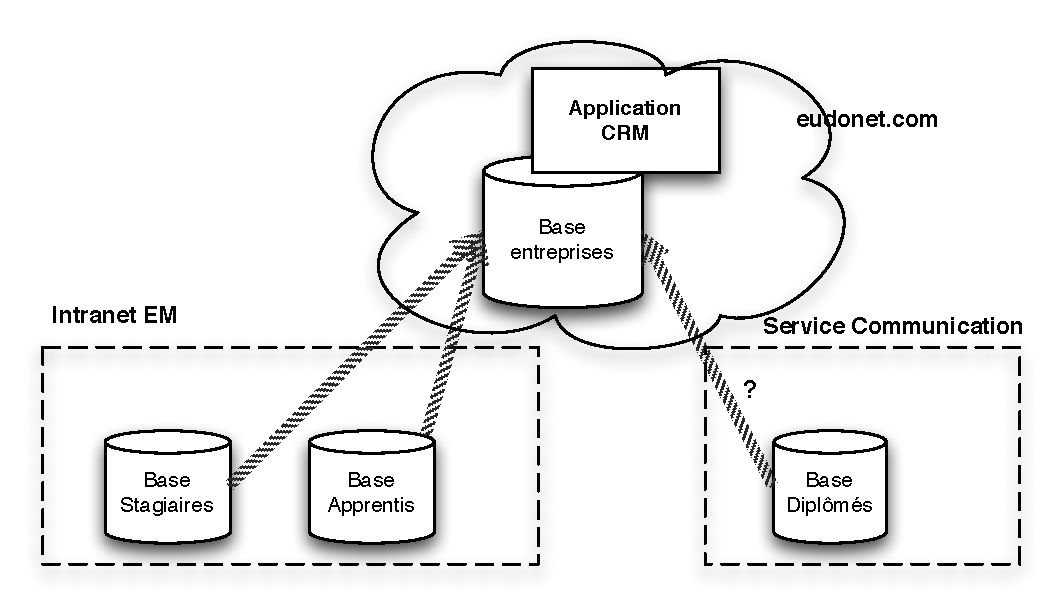
\includegraphics[width=.9\linewidth]{figs/crm_overview.pdf}
\end{center}
\caption{Positionnement du CRM dans le système d'information de l'EM}
\label{fg:crm_overview}
\end{figure}



%---------------  Communication  -----------------------------------
\section{Service communication}

\paragraph{Michèle Schmidt (MS), Isabelle Suhr (IS), Marine Julien (MJ), 
Nicolas Beyhurst (NB).}

\subsection{Processus fonctionnels}
Les processus nécessitant le support du système d'information peuvent 
être rangés en quatre catégories:
\begin{itemize}
\item[$\bullet$] SC1) La communication d'informations à des publics ciblés.
\item[$\bullet$] SC2) La gestion technique d'évènementiels.
\item[$\bullet$] SC3) La collecte d'informations pour répondre aux enquêtes de type 
      palmarès.
\item[$\bullet$] SC4) L'analyse de l'attractivité de chaque formation académique.
\end{itemize}
\bigskip

Dans la catégorie SC1) le besoin est de constuire des \textbf{listes 
pertinentes et ciblées d'adresses electroniques}. La difficulté
est bien sûr différente selon que la communication est à destination
d'un public interne ou externe à l'établissement.

En interne, il est nécessaire de disposer d'un \textbf{annuaire}
fiable et précis du personnel et des étudiants. 

Pour la communication vers l'extérieur, le mailing est souvent 
fait de manière indirecte : l'information à communiquer transite par
le service en charge du public visé, avec un contrôle informel des 
destinataires par le service en question. Ainsi, une invitation à un 
colloque académique sera transmise par Karine Bouvier (Recherche),
une invitation à un carrefour métier sera transmise par Bernadette 
Fischbach (Relations Entreprises) ou une information aux étudiants
est transmise à la scolarité concernée pour redifusion. La communication 
vers l'extérieur nécessite donc une \textbf{base de prospects} fiable 
qui puisse être consolidée avec les données d'autres services (scolarité, 
relation entreprises, recherche), ainsi que des \textbf{procédures 
de collectes} de nouveaux prospects le plus automatisées possibles.\\

Dans la catégorie SC2) on trouve en particulier l'activité de création
de mini-sites web par NB permettant de gérer chaque évènement (inscriptions,
programmes, informations pratiques, etc) ou du site des diplômés (alumnis).
Cette activité ne dépend pas du système d'information excepté pour
la mise à jour de l'annuaire des diplômés. Elle est au contraire 
support à la catégorie SC1) en fournissant les données déposées par les
visiteurs sur les sites web.\\ 

La catégorie SC3) nécessite de rassembler des statistiques provenant de 
nombreuses sources. Les informations à collecter et les services qui les 
produisent sont présentés en figure~\ref{fg:comm_flux}.
\begin{figure}[hbt]
\begin{center}
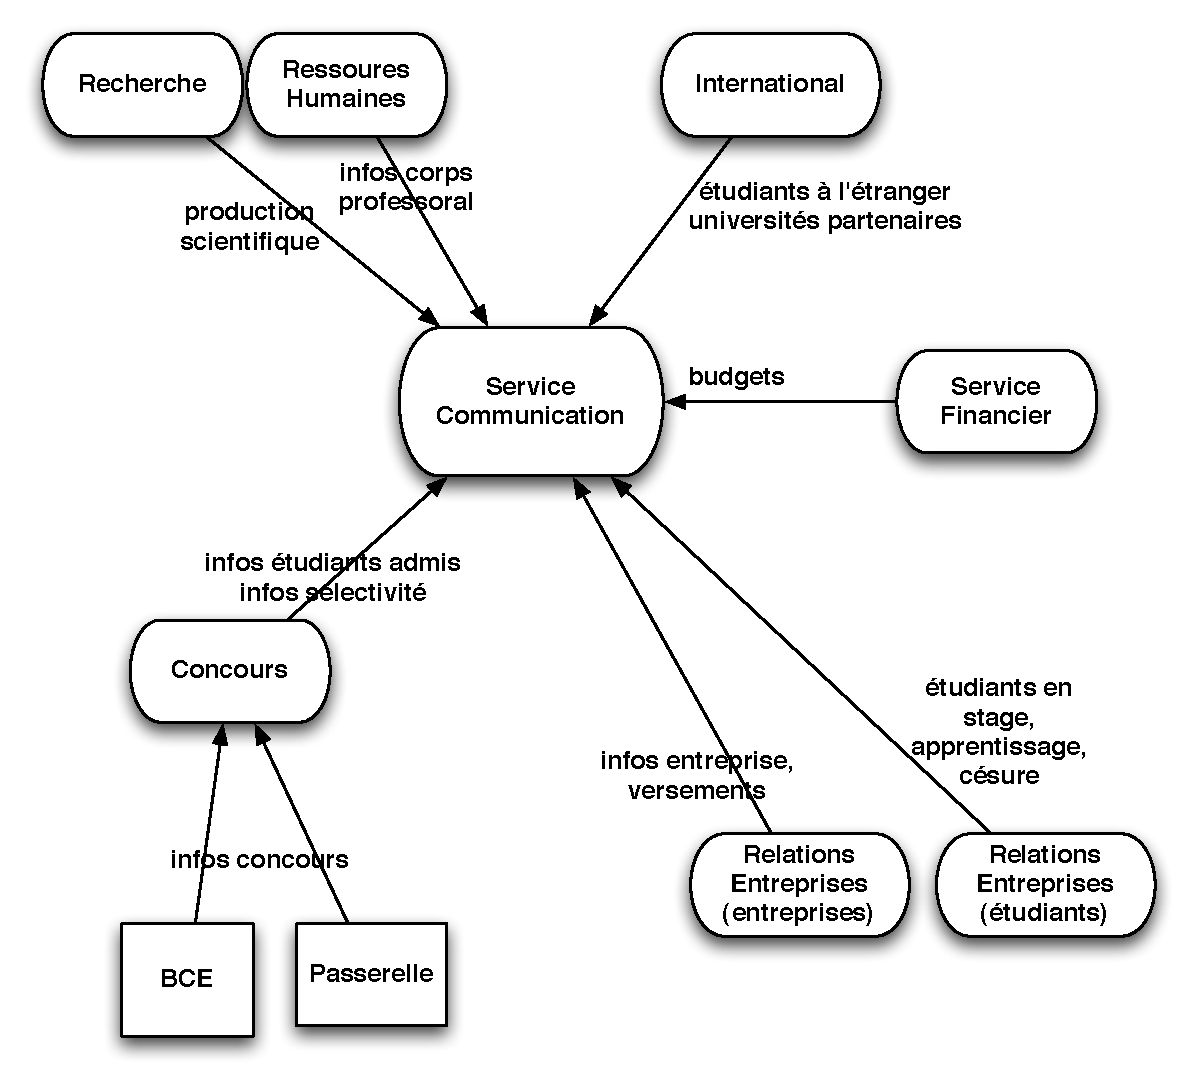
\includegraphics[width=.75\linewidth]{figs/comm_flux.pdf}
\end{center}
\caption{Les flux d'informations nécessaires pour répondre aux enquêtes de type palmarès}
\label{fg:comm_flux}
\end{figure}
Dans ces enquêtes, MS sépare les différentes questions posées et délègue
dans les services appropriés la charge de trouver l'information.\\


Dans la catégorie SC4), on compte les deux enquêtes intégrés (PGE et Master 
Universitaires, formation continue) qui apportent de l'information sur la 
typologie des étudiants nouvellement recrutés et la façon dont ils ont eu 
connaissance de l'établissement et de la formation. Cette information permet 
au service de mieux comprendre l'impact des différents supports de communication.

Rentre également dans cette catégorie les statistiques sur les formations
Master et EE à tous les stades du recrutement. IS a construit au cours 
des années un historique de ces statistiques, formation par formation,
et peut ainsi mieux analyser l'attractivité de chacune des formations.
Ces données permettent aussi d'ajuster les opérations de communication.
Par exemple, un nombre plus faible de demandes de dossier d'inscription 
à une formation peut suggérer une opération de communication ciblée.
Pour collecter ces statistiques, une synthèse des données était auparavant
demandée (via fichier partagé en réseau) à la scolarité aux différents 
étapes du recrutement (nombre de dossiers demandés, dossiers reçus, 
dossiers acceptés). 
L'accroissement du nombre de formations et la mise en place d'ARIA rend 
cette procédure caduque. Aujourd'hui, ces données dont récupérées
directement d'ARIA mais la précision est plus faible et ARIA ne 
conserve que les pré-inscriptions pour l'année en cours. Il faudrait
donc disposer d'un stockage auxiliaire pour fabriquer un historique.


\subsection{Existant}
\begin{itemize}
\item Pour les processus de catégorie i) pour la communication interne
	les données d'annuaire fournies par l'intranet EM %
	\footnote{\url{http://intranet.em-strasbourg.eu/adm/fr/grh/coordonnees.html}}
	sont utilisées de manière efficace pour communiquer par mail.
	En revanche, il n'existe pas d'annuaire plus complet permettant
	par exemple de connaître les fonctions et les status  (problème d'édition des 
	cartes de visites en français et anglais).


	Pour les processus de catégorie SC1) pour la communication externe,
	il existe des fichiers prospects dispersés et conservés dans des 
	formats techniques de stockage différents. Le tableau en figure 
	\ref{fg:comm_prospects} liste ces différents fichiers.
	L'utilisation de fichiers excel est la plus courante et considérée 
	la plus pratique actuellement.

\begin{figure}[hbt]
\begin{center}
	\begin{tabular}{llll}
	\hline
	\hline
	public	& source	 & format de stockage \\
	\hline
	prospects par évènements & inscription sur  mini-sites &  base de données, export csv (excel)\\
	prospects formation continue  & pré-inscriptions ARIA & import csv \\
	prospects diplômés      & service diplômés &  import csv, puis base de \\
					&			 &  données gérée dans le service Comm. \\
	étudiants après CRD 	& données APOGEE & import csv \\
	journalistes 		& contact personnel	& carnets d'adresse \\
	salons, contacts divers	& contact mail, carte visite & carnets d'adresse, fichiers excel\\ 
	VIP institutionnels	& contact mail, carte visite & carnets d'adresse, fichiers excel\\ 
	\hline
	\hline
	\end{tabular}
\end{center}
\caption{Fichiers prospects utilisés pour communiquer vers l'extérieur, source 
	d'acquisition et format de stockage}
\label{fg:comm_prospects}
\end{figure}
	Ceux-ci  ont pu être constitués par la collecte des informations saisies 
	par un participantà un évènement (inscription sur mini-site), ou lors de 
      salons (saisie manuelle). L'application ARIA de pré-candidature (application de l'UdS)
      peut aussi être utilisée pour produire des fichiers prospects (personnes 
	ayant entamé une démarche d'inscription sans finaliser).

\item Dans la catégorie SC2) NB développe de manière réactive des sites couplés à 
	des base de données selon des formats ouverts (logiciels libres PHP, MySQL) 
	qui répondent aux besoins ponctuels de gestion d'un évènement, permettant
	de conserver de manière pérenne ces données. Son action est cependant intrinsèquement
	limitée par la difficile connexion à d'autres sources d'informations (intranet 
	EM et applications du S.I. UdS).

\item Dans la catégorie SC3) les données ne sont pas stockées mais simplement reportées
	aux demandeurs dans le format souhaité.

\item Dans la catégorie SC4) les processus sont manuels et les données enregistrées
	dans des fichiers personnels.
\end{itemize}

\paragraph{Analyse}

D'une part, le service communication a globalement besoin d'informations 
réparties dans la quasi-totalité des applications du système d'information.
Aujourd'hui, la collecte des informations nécessaires est déléguée aux
services les plus proches de ces applications. Cependant, il est probable 
que ce fonctionnement serait recommandé même si le système d'information
était directement interrogeable par le service communication.

D'autre part, le service communication possède et produit ses propres
données, principalement des contacts. La gestion de ces données
est hétéroclite en raison des supports divers. La disponibilité de
l'information n'est pas totalement maîtrisée car certaines données peuvent
échapper aux sauvegardes car non entreposées dans des espaces de stockage
sauvegardés par les services informatiques). Les outils bureautiques utilisés
font que l'information est peu efficiente et peu efficace. 


Du point de vue des applications, la présence d'un informaticien au
sein du service aide considérablement à la résolution de problèmes
techniques ponctuels. Ceci ne peut cependant pas remplacer la mise
en place se solutions applicatives plus globales. Il manque en particulier
un outil pour faire du mailing de masse compatible avec les règles de
sécurité anti-spam de l'UdS. L'emploi d'outils collaboratifs adaptés 
permettrait également de gagner en efficacité. 


\paragraph{Bilan qualité des données}
~\\


	\begin{tabular}{|l|l|l|l|l|l|l|}
	\hline
	efficacité	& efficience &	confidentialité	& intégrité & disponibilité & conformité & fiabilité \\
	\hline
	
	\hline
	\end{tabular}
	

%------------------------------- R H -------------------------------------------------

\section{Ressources humaines}

\paragraph{Laurie Walbrou (LW), Emilie Kaës (EK)}


\subsection{Processus fonctionnels}
Les processus nécessitant le support du système d'information peuvent 
être rangés en deux catégories:
\begin{itemize}
\item[$\bullet$] RH-1) La gestion du personnel administratif et enseignant
\item[$\bullet$] RH-2) L'organisation d'évènements
\end{itemize}
\bigskip

La catégorie RH-1) représente l'immense majorité de l'activité.

Le besoin est de \textbf{collecter des informations pertinentes
sur le personnel} de l'EM. La pertinence se décline selon
deux besoins plus spécifiques:
\begin{itemize}
\item RH-1.1) les besoins pour répondre aux accréditations, enquêtes palmarès, 
	au label diversité, écrire le bilan social.
\item RH-1.2) les besoins issus du dialogue de gestion avec l'Université.
\end{itemize}

\bigskip

Le besoin RH-1.1) nécessite des informations très nombreuses, précises
et changeantes d'années en années. Ainsi l'accrédidation ACSB 
pourra demander pour chaque enseignant combien d'années il a passé
à l'étranger les cinq dernières années.
Ces contraintes spécifiques \textbf{obligent l'établissement à 
posséder une base propre} de ces informations étant les logiciels
de gestion de RH disponibles à l'UdS.\\

Le besoin RH-1.2) est beaucoup moins exigeant. Il fait appel à toutes
les informations administratives contenues dans HARPEGE et SOSIE
concernant les personnels.\\


Concernant les activités de la catégorie RH-2) le besoin exprimé 
est la mise en place d'un agenda partagé permettant d'éviter
les conflits de date lors d'organisations d'évènements, et de 
diffuser l'information évenementielle sans faire d'invitation
par mail mais par un mécanisme de publication/souscription
(e.g fil RSS, synchronisation d'agenda).  



\subsection{Existant}

Le processus correspondant au besoin RH-1.1) a conduit à mettre en
place une procédure pour le recrutement des vacataires. Cette procédure
est décrite par le diagramme de séquence en figure \ref{fg:rh_seq_vacataires}.
Elle vise à enregistrer les informations perinentes concernant les enseignants
au moment de la candidature en analysant le CV d'un candidat retenu. Ces
informations sont enregistrées dans un fichier Excel maintenu par EK.

\begin{figure}[hbt]
\begin{center}
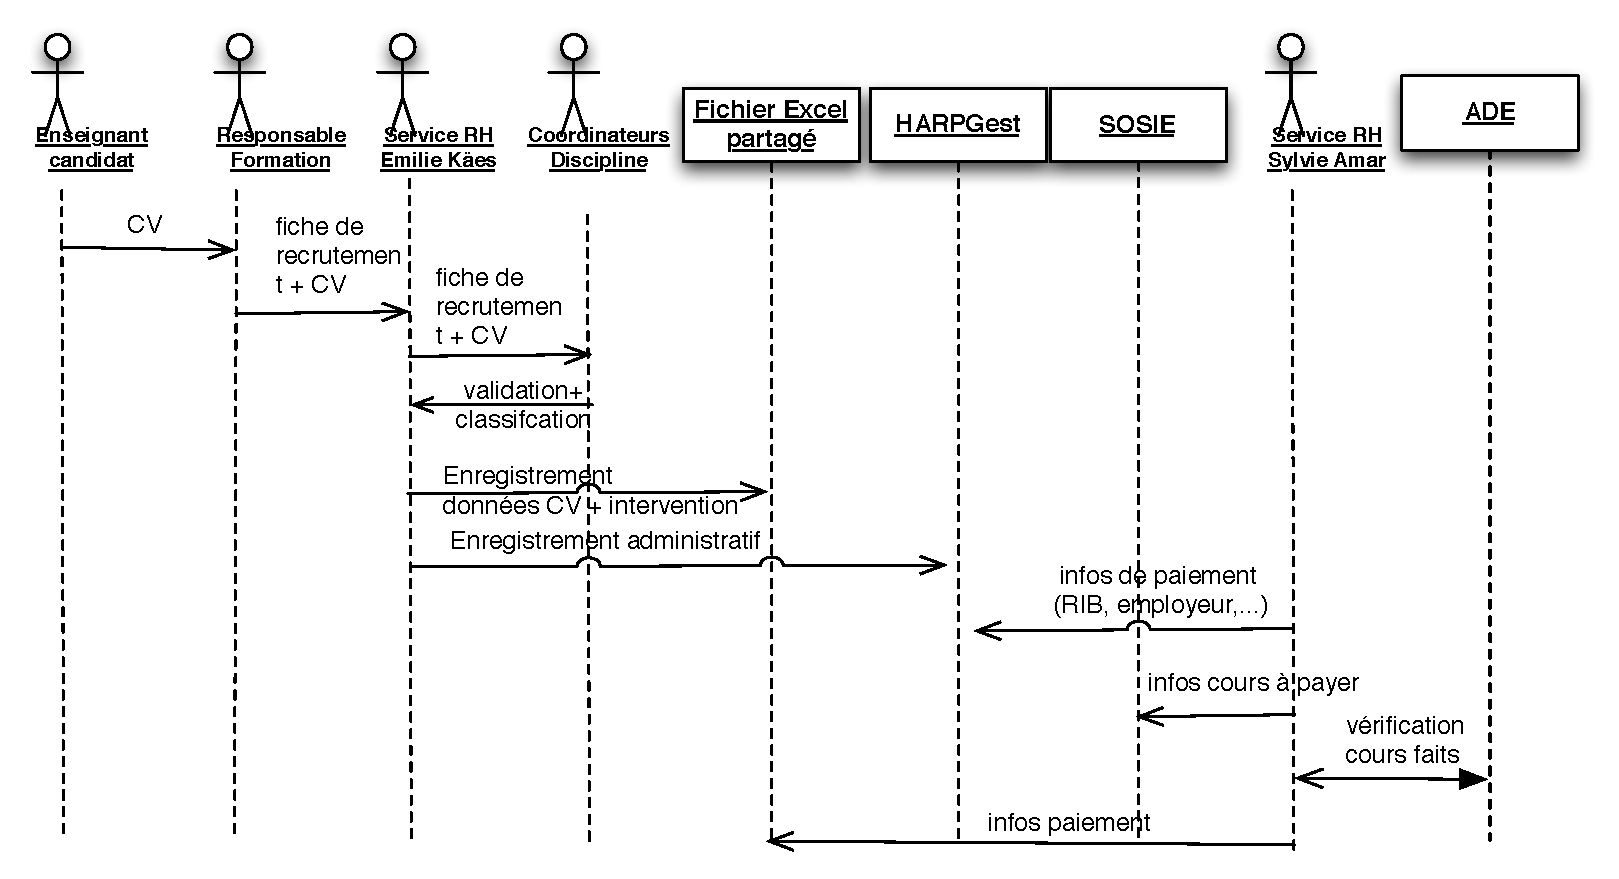
\includegraphics[width=\linewidth]{figs/rh_seq_vacataires.pdf}
\end{center}
\caption{Diagramme UML de séquence pour la procédure d'enregistrement d'un vacataire.}
\label{fg:rh_seq_vacataires}
\end{figure}

Le reste de la procédure vise à enregistrer administrativement l'enseignant
dans le S.I. de l'UdS: application SOSIE pour les heures effectuées et payées
et application HARPGest pour mémoriser les informations d'état civil et celles
nécessaire au paiement des heures. 
Cependant, ces \textbf{applications se révèlent totalement inefficaces} dans 
le reste du processus. Ainsi, les extractions d'HARPGest ne peuvent fournir
que les noms, date de naissance et nationalité d'une personne. SOSIE ne liste
que les heures de cours \emph{payées} et sur des intitulés de matière qui
peuvent avoir changé dans APOGEE.
Pour connaître l'état des paiements des heures, la procédure en place prévoit
que Sylvie Amar édite le fichier excel (partagé en réseau) pour y inscrire 
les heures payées pour chaque enseignant.\\

Les processus de la catégorie RH-1.2) subissent les mêmes manquements en terme
de support du système d'information. Le dialogue de gestion annuel implique
de faire à minima un état des lieux précis des personnels permanents de 
l'établissement. Cependant, les applications en place ne permettent même pas
d'obtenir les numéros de postes sur lesquels les personnes sont en place.
LW maintient son propre fichier pour ces postes. Elle obtient cette information
par contact téléphonique auprès d'une responsable au service RH de l'UdS, et
non sur la base d'une importation automatique de données.\\

Concernant le besoin RH-2.), aucun outil n'est aujourd'hui en place.

\subsection{Analyse}

Le support du S.I. aux RH est en train d'évoluer. Avant la mise en place
de la procédure décrite (figure~\ref{fg:rh_seq_vacataires}), et relativement 
aux processus décrits ici, le service RH fonctionnait sans aucun support réel 
du point de vue des systèmes d'information. La perspective de créer un outil 
spécifique pour gérer les candidatures et CV a été évoquée dès 2006 mais ne 
s'est pas réalisée. 
Confrontés aux demandes des accréditations, en 2009, le service RH a passé
de l'ordre de 10 mois hommes (quatre personnes en janvier, février, mars)
pour analyser les CV papiers des enseignants intervenant (de l'ordre de 500). 
Un nouveau projet a été conçu, intitulé \textit{Base de 
données CV}, dont le document de travail est copié en annexe~\ref{ch:rh-cvtheque}.
Idéalement, ce projet devrait mis en production en décembre 2011. 
Cependant, le manque général de planification des projets et la faible 
formalisation du cahier des charges pourrait rendre cette échéance improbable.\\

La procédure actuelle est adaptée aux demandes et devrait permettre de 
répondre assez efficacement aux questions. Cependant, le fichier excel
dans lequel figure quasiment toutes les données est le point névralgique
de ce processus, et à ce titre représente un risque certain. Etant sur
un espace commun, il est censé%
\footnote{Vérification non effectuée lors de l'audit.}
être sauvegardé par le service informatique mais la gestion des droits
étant difficile, on peut imaginer qu'un autre administratif corrompe 
(y compris non-intentionnellement) les données y figurant.\\

Concernant les applications, il faut retenir que les applications
du S.I. de l'Université ne fournissent quasiment aucune information en
retour (SOSIE et HARPGest). L'ADE permet de vérifier les cours effectuées.
L'intranet EM n'est pas du tout utilisé par le service RH.
 

\section{Executive Education }
Pia Imbs (Directrice déléguée)

\section{Accréditations}
Maxime Merli, Fatiha Boutera

\section{Concours }
Aida Saïd, responsable

\section{Masters Universitaires}
Géraldine Broye (Directrice déléguée),

 
\section{Scolarités}

\section{Programme Grande Ecole}
Babak Mehmanpazir, (Directeur déléguée)

\section{Service International}

\section{Université numérique}


%----------------------- ----------------------------------------------

\chapter{Analyse}

 - pb interlocuteur

- pb planification projets / travailler mode projet 

- doubler les personnes sur les tâches critiques

- les personnels informatique se sentent entravés vis-à-vis de la DI

- les personnels informatique ne travaillent pas ensemble

Dépendent de l'intranet historique de l'IECS (CK)
- annuaire personnel EM + vacataire


%----------------------- BIBLIO ----------------------------------------------
\bibliographystyle{alpha}
\bibliography{biblio}
%----------------------- ANNEXES -------------------------------------
\appendix

\chapter{Cahier des charges du CRM}
\label{ch:annexe-crm}
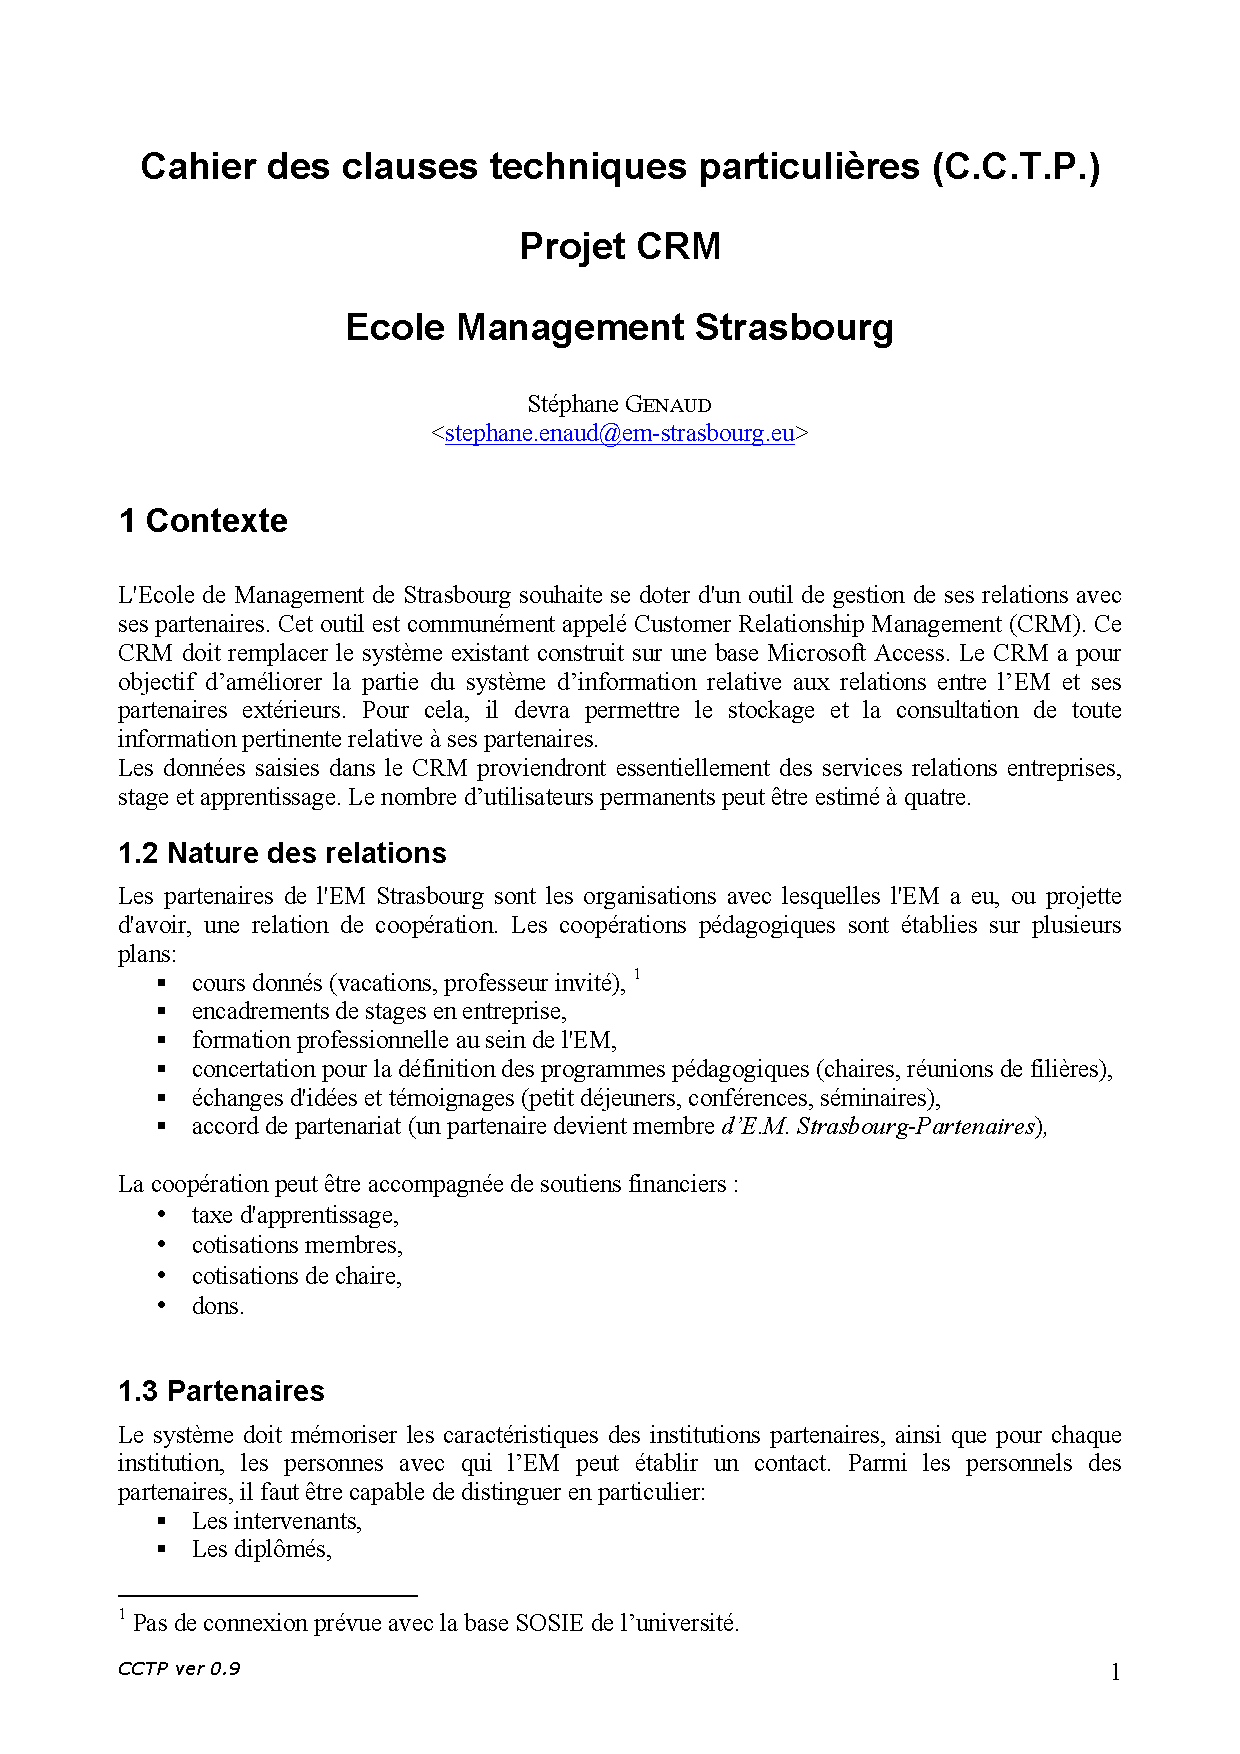
\includepdf[pages=1-5]{figs/crm_cctp.pdf}


\chapter{Descriptif demande pour la CVthèque}
\label{ch:rh-cvtheque}


\printindex
\end{document}

 
  
 

